\chapter{PRELIMINARY DIAGNOSIS}\label{PRELIMINARY DIAGNOSIS}

\section*{IDENTIFICATION OF THE 5 SYSTEMS}
The Viable Systems Model is based on 5 systems which are seen as fundamental to viability.

If all 5 systems are working well within you organisation, then you can say that the basic functions needed for viability are present. If they are not, then your organisation is not viable in the terms defined in this pack, and you will need to change your organisation to ensure viability.

The purpose of the Preliminary Diagnosis is to identify the 5 systems needed to ensure viability, and to draw them on a large VSM diagram which represents the parts of your organisation in its totality.

If any are not present, they will need to be designed and added to your organisational structure.

If any existing parts of your organisation do not fit into one of the 5 Systems, then they are not crucial for viability and may be unnecessary.

\section*{Preliminary Diagnosis - How it Works}
I was told this story by a colleague (referred to as GB) who lectures in Management Studies, and who uses the VSM as a tool in his consultancies. It gives such a clear picture of the use of Preliminary Diagnosis that I decided to include it at this point.

He was telephoned one morning in connection with the proposed amalgamation of several businesses into an alliance designed to enable the member companies to combine their strengths, and thus compete more effectively in exporting their products. The group had done some preparatory work, but needed advice quickly. A meeting was scheduled for 2.00 pm that afternoon.

Usually, a consultant needs several days to assess the situation and gather the background which is essential for sound advice.

This was clearly impossible.

So, GB arrived for the first meeting with a large piece of paper on which was drawn the outline of the VSM, that is the Operational units and Systems 2, 3, 4 and 5.

As the meeting proceeded, he began to ask questions about the proposed organisation and to fill in the boxes in his VSM diagram. Operational units: the member companies. And so on.

After the proposed organisation had been described, some of the boxes were empty and GB began to probe "How do you intend to ensure that the member companies work together in a more effective manner - won't you need someone to examine the various possibilities and to look for synergy?"

Basically, he was looking for something to write in the System 3 box.

This is the essence of the Preliminary Diagnosis. You define a function, look for the bits of your own enterprise which does it, and write it in on the relevant part of the diagram.

The VSM is so thorough in its model of how a business works, that GB's clients were overwhelmed with "his" insight and made aware there were several aspects of the organisation they had completely overlooked.

And all of this without any preparation.

In your case, assuming you are looking at an existing business, the insights are unlikely to be so staggering. Problems with viability will have arisen and been dealt with, and somewhere the functions needed for viability will have been implemented. The question is - are they adequate?

But whatever the context, you will be mapping your own organisation onto a VSM diagram, and this process is bound to affect the way you look at your enterprise.

\section*{Step 1: DEFINE THE SYSTEM TO BE DIAGNOSED}
\textbf{PURPOSE: To clarify the boundaries of the System-in-Focus.}

During the diagnosis which follows, there are times when it's easy to lose track of exactly what is being studied. So its essential to begin the Preliminary Diagnosis with a clear statement of the organisation (or the parts of the organisation) you are looking at. Throughout this guide, this will be referred to as the System-in-Focus.

Before starting the Diagnosis and the identification of the systems needed for viability, you should list all the parts of the System-in-Focus as you see them.

The list should be exhaustive as it will be referred to throughout the Preliminary Diagnosis. It will contain the Operational parts, the accounting functions, the management functions and so on.

In compiling the list, keep one eye on your sketch of the various recursions and ensure that the items on the list refer only to the system-in-focus. It's likely that your first list will need revision and that one or two items will belong to another recursion. Check it carefully.

As the Preliminary Diagnosis proceeds, you will be able to take the items on your list and allocate them to one or other of the 5 systems within the Viable Systems Model. Thus, the list will gradually disappear.

If your organisation is perfectly Viable, the list will disappear completely and there will be 5 well defined systems giving the basis for viability.

If not, either

\begin{itemize}
  \item some new jobs may have to invented
\end{itemize}

or

\begin{itemize}
  \item some existing jobs are not needed for viability and can therefore be considered as redundant.
\end{itemize}

\section*{Step 2: DRAW THE VIABLE SYSTEM MODEL IN OUTLINE}
The diagnosis of your organisation will proceed by drawing a large diagram which will represent your System-in-Focus as a whole system. At this stage, the outlines of the three main parts of the VSM - Operation, Metasystem and Environment - will be sketched in. Between them they represent the overview of your System-in-Focus in its totality.


\section*{DRAWING THE VSM - from Step 2 - drawing the outlines}
\textbf{Notes:}

\begin{enumerate}
  \item There is a tendency to see this diagram as hierarchical. The Boss over the Workers. From my experience, (and from discussions with Beer) this is completely wrong. The Metasystem is there to service the Operational elements. It has a different perspective, or over-view, as it has to consider the collection of Operational units in its entirety, but the need to have power over the people in the Operation is strictly limited to its job of cohesion. It can only wield power if the system is in danger of breaking apart.

  \item Everything which will be drawn on this diagram must refer to the System-in-Focus. At a later stage you may want to delve further into the workings of each Operational element, so you will drop a level of recursion, define a new system-in-focus and start again. For the time being the diagnosis will concentrate upon the System-in-Focus you have defined.

\end{enumerate}

\section*{Step 3: SYSTEM ONE - THE OPERATION}
\textbf{PURPOSE:} To specify those parts of the system-in-focus which undertake System One (primary) activities.

The first system in the Viable Systems Model is the entire Operation which will be composed of several Operational units.

The Operational units undertake the System-in-Focus's basic activities.

They will all be (smaller) Viable Systems in themselves, and thus must be able to maintain a separate existence.

System One generates wealth and in a business, each element can be considered as a profit centre.

If you are a manufacturing business, System One is the production units, the teams of people and machines which actually do the manufacturing.

If you are a programming co-op, System One is the programmers or teams of programmers, perhaps divided into various specialist areas.

If you are looking at a more complex organisation, you may have a System One which includes manufacturing, distribution, and warehousing.

System One sounds straightforward, but is actually one of the most difficult areas to define clearly. For example, in the examples given above the computer department was a System One in the programming firm, but the computer department in the manufacturing company would have a support role and would therefore not be part of System One. Some people who are in basically service areas such as engineering maintenance may consider themselves important enough to be System One.

The question is: are they part of what the organisation is really about, or are they back-up, facilitators, or support? If the answer is the latter, then they do not qualify as System One.

You are now in a position to go back to the original list of jobs carried out by your System-in-Focus, and to list those which between them make up System One.

Note: Each Operational unit is a VSM at the next recursion down and thus will include both the physical aspects and the management of one aspect of the Operation. So, for example, the trucks and drivers and the management of the transport department are found within that Operational Unit.)

\section*{DRAWING THE VSM - from Step 3 - adding the Operational Units}
\begin{center}
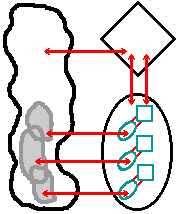
\includegraphics[max width=\textwidth]{3vsm_aou}
\end{center}

This diagram shows the VSM with three Operational units high-lighted.

There is no reason why you should have three, although it is unlikely that you have more than eight.

The diagram also shows the parts of the environment which are specific to the Operational units.


\section*{Steps 1, 2 and 3: Example}
\begin{center}
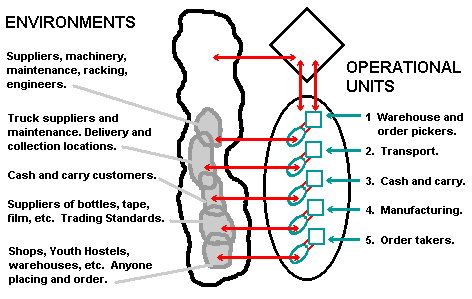
\includegraphics[max width=\textwidth]{3suma}
\end{center}

So far you have drawn the VSM in outline and added

\begin{itemize}
  \item the Operational units

  \item the external environments which are specific to each of the Operational units.

\end{itemize}

At this stage the Suma VSM looked as follows:

SYSTEM IN FOCUS: Suma Natural Food Wholesalers

MISSION: Warehousing and Distributing Natural \& Ecological products.


\section*{Steps 1, 2 and 3: Another Example}
\href{http://www.radicalroutes.org.uk/}{Radical Routes} is a group of co-operatives in the UK who have formed a loose Federation in order to promote their activities.

They found the VSM an interesting environment with which to look at their problems and carried out a Preliminary Diagnosis on their own.

They began with System One and thought \textit{So what are we really about ... what are the primary activities?} Understandably, they began to draw the Operational elements as the activities of the federation; for example fund-raising, education, stimulating interest about co-operatives and so on.

I was then invited to meet with them and discuss the work they had done.

After some discussion we decided that a more useful way of looking at System One was as follows:

\begin{itemize}
  \item Radical Routes exists to service the member co-ops

  \item The primary activities of Radical Routes concern the member co-operatives themselves

  \item Therefore the Operational units are the member co-operatives and all the activities of the federative body are Metasystemic.

\end{itemize}

After this fundamental re-think we spent the rest of the afternoon looking at the design of the whole system in these terms.

A diagnosis based on the original definition of System One would have come up with entirely different results.

So please note:

\begin{enumerate}
  \item The way that you define the Operational elements largely determines the way that the rest of the diagnosis proceeds.

  \item This is crucial to a useful outcome. The Operational parts need to be primarily concerned with their own internal issues (minding their own business) while the Metasystem parts can only function if they have the ability to prioritise the over-view. If these are wrongly chosen, then the system cannot function effectively.

  \item There are no absolute rights and wrongs. A model is only correct to the extent it is useful. Radical Routes may well have reached interesting conclusions from their initial guess, and only the final outcome (did it work?) can judge which diagnosis was the better. Pause for breath .....

\end{enumerate}

At this stage it is sensible to review what's happened so far, and to think about how the Preliminary Diagnosis is going to proceed.

So Far ...

You have drawn in outline three shapes which represent your System-in-Focus in its totality, and its external environment.

You have defined your System-in-Focus and its Mission Statement.

The System-in-Focus has been defined in two parts:

\begin{enumerate}
  \item The Operational units which carry out the primary activities, which DO whatever is needed to fulfil the Mission Statement. and ...

  \item The Metasystem which is there to provide whatever services are needed by the Operational units to ensure they hang together in an integrated form.

\end{enumerate}

You have listed all the parts of your enterprise which are part of the system-in-focus as you see them.

You have extracted the parts which between them make up the Operation or System One.

You have drawn these Operational units on the outlined VSM with their corresponding local environments.

The Next Stage ...

Having listed the Operational units in System One, you will be moving on to look at the Metasystem, and it is important to bear in mind the following thoughts:

\begin{enumerate}
  \item The Metasystem is charged with doing whatever is needed to enable the Operational units to come together to make a single, integrated, coherent system. It may be defined as providing the "glue" to make sure the autonomous departments don't drift apart into a number of isolated bits.

  \item The Metasystem will always be concerned with the Operation as a whole. It may be looking at the interactions between the Operational units or at the implications of a policy decision, but at all times it is involved with System One in its entirety.

  \item It will not be concerned with internal matters within the Operational units. This would be comparable to expecting you to be involved with the mechanics of the beating of your heart. In general the Operational units are seen as autonomous and the Metasystem is concerned only with the way they interact.

\end{enumerate}

\section*{Step 4: SYSTEM TWO - STABILITY AND CONFLICT RESOLUTION}
\textbf{PURPOSE:} To identify those parts of the System-in-Focus which ensure that the Operational units interact in a stable manner.

\subsection*{Why think about stability?}
Without exception, all systems with interactive parts, regardless of their nature, have stability problems.

Anyone who's had the misfortune of trying to ride a bicycle with a buckled wheel down a steep hill will know how an unstable system can behave, and why the consideration of stability criteria is an essential part of any design.

Instabilities between people are just as universal. Look at young children in the playground, or marital break-down, or the way communes inevitably collapse.

Nation States exhibit extreme instabilities, the arms-race being the most concerning outcome.

But whatever the particular case, the need for some way of dealing with instabilities is essential, otherwise the organisation will shake itself to pieces.

The argument goes:

\begin{enumerate}
  \item The parts of a system will invariably have conflicting interests.

  \item These conflicts will tend to lead to instabilities.

  \item Instabilities left unchecked become destructive, and the system will begin to oscillate. (I want it! Give it to me! No I won't!)

  \item To deal with this, any viable system must have a System Two for:

\end{enumerate}

\begin{itemize}
  \item resolving conflicts

  \item dealing with instability

  \item damping oscillations

\end{itemize}

\section*{A System 2 story}
Suma used to have a three floor warehouse in which goods were moved up and down by fork trucks lifting pallets through holes in the floor. Every now and again, a pallet would fail to find a home and the top floor operator would send the pallet back down to the middle floor. The operator on the middle floor would think "this isn't my pallet - it will have to move back up" and the pallet would go up and down, up and down, all day.

The motion of the pallet was exactly like a yo-yo, or in Beer's terms it was oscillating due to conflicting interests between Operational elements.

The resolution of this problem was to get the operators from each floor to meet, to discuss the problem and then to resolve it: "Look someone has to agree to take this pallet and its definitely nothing to do with me - I only do beans and grains." "Yes, but you're the only one with enough spare space ... my floor's too full already" Eventually agreement was reached, the pallet was found a home and the oscillation stopped.

A general strategy for System Two in this context would be a series of rules for allocating pallets. If it were thorough enough, oscillations would be rare.

Beer lists many examples of instabilities in industry which lead to oscillations. One of these came from his observation that the stocks of raw materials in a production shop vary dramatically. Sometimes they run so low that everyone is worried that they will run out, sometimes they are so high that the available space runs out and storage becomes a problem.

The stock levels oscillate between these extremes. Again a System Two needs to be designed to stabilise this situation, for example Just In Time ordering, which keep inter-process stocks to a minimum.

In some cases System Two may be a nuts-and-bolts system like a production schedule or a timetable which will ensure that conflicts do not arise as several parts of an organisation are all clamouring for the same resources.

In other cases, System Two may be more subtle. In Mondragon the predominant System Two was the methods they employed to share resources and support each other's businesses. My attempts to find out how they deal with conflicts between competing businesses were always answered with "but we share all profits anyway ... why should there be a problem?" In the case studies which you read you will notice that System Two in a co-operative is generally covered by the "co-operative ethos." It seems clear that in an organisation in which the common good is paramount, instabilities will be fairly easy to resolve.

If the company ethos is competitive, if your success is measured against the performance of others, then it's much more likely that your interests will be exactly the opposite of others. So the temptation will be to act in such a way that your successes will bring about others' failures. And of course everyone else is doing the same.

Obviously, a co-operative will not be completely free of this kind of thing: there is only so much money to spend and the various Operational elements will compete for it. Some people are naturally competitive. Cash flow will need to be controlled. The financial System Two will have to be designed.

However, in most of my applications, working within a co-operative ethos means that there is already a pervasive System Two, and this gives the System two designer a head start.

\section*{Summary}
System Two is charged with dealing with the instabilities which inevitably arise between the Operational units.

Every organisation must have a System Two:

\begin{itemize}
  \item to resolve conflict

  \item to deal with instabilities

  \item to damp oscillations

\end{itemize}

\section*{DRAWING THE VSM - from Step 4 - adding System Two}
\begin{center}
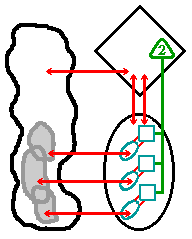
\includegraphics[max width=\textwidth]{3vsm_as2}
\end{center}

The diagram to the right shows the VSM with System 2 added (in green).

Note that System Two is part of the Metasystem (it sits in the diamond) and that it passes through every Operational unit.

Thus, it looks at the entire collection of interacting System One units with a view to resolving conflicts, dealing with problems and creating stability.

System Two has been drawn slightly larger than usual for emphasis.


\section*{Step 4: IDENTIFICATION OF SYSTEM TWO - examples}
You have now drawn in System Two on the VSM diagram.

Examples of System Two are as follows:

\subsection*{System Two: Suma}
System Two is generally performed by the co-operative ethos which prevents major conflicts between members.

The weekly Rota allocates members to various jobs according to departmental needs, and thus stabilises the problem of too many people in one area and not enough in another.

There must be good cash flow control, thus stabilising the tendency for huge surpluses and overdrafts.

The recent stock-control system stabilises stock holdings and avoids an oscillation between vast stocks and goods going out-of-stock.

\subsection*{System Two: Mondragon}
Mondragon provides a System Two by sharing profits and by mutual financial support. This resolves any conflict of one business benefiting at the expense of another.

\subsection*{System Two: School}
The timetable is regularly cited as the ideal System Two.

It takes care of double-booking, and resolves the conflict of several teachers all wanting the same rooms, projectors etc., etc.

\subsection*{System Two: Manufacturing Company.}
System Two is the production schedule which performs the same stabilising function as the school timetable. It resolves the conflict which could emerge in competition for limited resources.

\section*{Step 5: SYSTEM THREE - OPTIMISATION}
\textbf{PURPOSE:} To identify those parts of the System-in-Focus which optimise the interaction of the Operational units, and to update the VSM diagram accordingly.

\section*{A System Three Story}
Consider a Viable System consisting of several dozen people trying to put out a fire by running to a nearby lake, filling a bucket and running back to throw the water on the fire.

Each person with a bucket is an Operational unit. Each will be absorbed with his own job.

The Metasystem - which may be one person sitting on the top of a ladder - will look at the whole system and may say "Keep to the left on the way down" (\textit{System 2} - stopping continuous collisions) or it may think about optimisation.

Eventually she may realise that if everyone forms a chain and moves the buckets from hand to hand, then you only have to move the water and buckets, and not your own body weight. The same job can be done, but only a fraction of the energy needs to be expended.

The extra efficiency which is generated as a consequence of acting as a whole system rather than an un-coordinated collection of parts is called synergy, and the generation of synergy is the essence of System Three.

\section*{The Job of System Three}
In all cases, System Three has the same function:

\begin{itemize}
  \item It is poised with an over-view of the entire collection of Operational elements.

  \item It looks at the way these elements interact.

  \item It considers way of optimising the overall efficiency of the entire collection of Operational elements.

  \item This improvement in efficiency is called synergy, so System Three's job is usually described as generating synergy.

\end{itemize}

Synergy is of course the essence of co-operation: four people working together co-operatively may be twice as efficient as four people doing the same work on their own.

The current task is to describe the ways that System Three functions within a viable system.

\begin{itemize}
  \item How does it deal with the Inside and Now?

  \item What does it do to generate synergy?

\end{itemize}

\section*{System Three - the Diagrams.}
\begin{center}
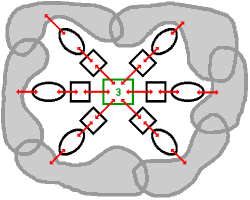
\includegraphics[max width=\textwidth]{s3_ool}
\end{center}

System Three is best thought of in the middle of a whole lot of activity. All around it the Operational elements are concerned with meeting the demands of their own environments (answering the phone, getting the orders completed on time, scheduling the trucks ...) and interacting with each other.

System Three sits right in the middle of all this activity, thinking about ways of optimising the whole thing.

Although this depicts nicely the relationship between Systems Three and One, it's a bit messy, and leave no room to illustrate the interactions between System Three and the rest of the Metasystem.

So \textbf{it's usually drawn above a stack of Operation elements like this}:

\begin{center}
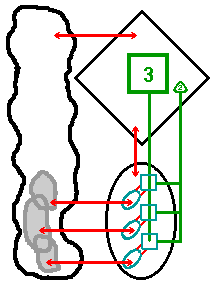
\includegraphics[max width=\textwidth]{3vsm_as3}
\end{center}

This diagram shows the VSM with System 2, reduced to fit into the Metasystem's diamond and outlined, and a large System 3 added for emphasis.

It's shown interacting with three Operational elements, although not as clearly as in the first diagram.

This arrangement has much more in common with the human System Three - the base brain - which sits on top of the spinal column and optimises the working of the muscles and organs.

We can now begin to describe the ways in which System Three over-sees the collection of Operational elements, looking for synergy.

\section*{The Resource Bargain}
System Three usually controls the purse strings. Resources are ultimately limited, and so it's essential for System Three to allocate them according to the global needs of the System-in-Focus.

This requires System Three to look at the whole of System One, and to allocate resources so as to optimise performance.

Thus System Three may say: "Your job is to get the goods to the customers in the most effective way, and we will give you £200,000 a month to do it. And as long as you do the job properly, you will continue to get the money."

Obviously this will require lots of negotiations between all the Operational units and System Three, and it leaves System Three with enormous amounts of flexibility to generate synergy "Hmmmm .... if I put a few more resources into production they say they can be 17\% more efficient. But that will mean cutting back on procurement and cut our margins by 1.52\%. On balance that looks fine ...a much better allocation of resources."

In a team, the resource bargain is more likely to involve allocation of people. "You do this and I'll do that, and things will work better ..." In a jazz band it could be allocation of time "The sax solo went on longer than expected, I'll cut down my break on keyboards."

But whatever the particular example, manipulation of the resource bargain provides a means of optimisation.

\section*{Operational Accountability}
Once an Operational unit has been allocated its share of resources, it must demonstrate that it's using them properly.

Thus the Operational elements must be accountable: they must be able to show that everything is proceeding as agreed with the Metasystem.

This is an essential aspect of the resource bargain; it's the way the Operational element demonstrates that it can justify the continuing allocation of resources from System Three.

The human Viable System has without doubt the most thorough network for demonstrating that all is going well. Every part of the body sends continuous messages to the base brain which knows just what's going on in real time. During periods of intense activity, this information is used by the base brain to modify the flow of adrenaline to the organs and muscles to optimise their operation.

Beer's design for an equivalent system in an enterprise is based upon near real-time monitoring of all System One activity and a set of statistical filters assessing the information. The System Three office would have a big green light or a continuous tone which would mean "everything is OK". As soon as any of the measurements moved outside acceptable limits, the light would go off, and other signals would identify the source of the problem.

But whatever the design, the Operational units must have a way of justifying their allocation of resources.

\section*{The Command Channel (1): Intervention Rules.}
Inevitably there will be problems. What happens if one Operational unit begins to deteriorate due to machinery breakdowns, all the trained personnel leaving suddenly, or something completely unexpected like a flood? In some cases the unit can cope, in others it may not and this may threaten the survival of the entire enterprise.

Clearly, there must be rules in place to deal with this. In certain situations System Three has to be given the mandate to intervene within an Operational element.

For example, if the information shows that productivity is down, wastage is up and morale has collapsed, then it's essential for System Three to intervene. Intervention means loss of autonomy and is only permitted when the cohesion of the whole system is at risk.

Intervention rules must be defined clearly, so that each Operational element knows it will be left alone unless it transgresses the agreed norms.

All of this needs careful design.

Beer has a simple recipe for deciding on the level of autonomy which can be allocated to an Operational element . He says autonomy should only be forfeit when system cohesion is at risk. So, if the actions of one Operational unit threaten to shake apart the whole system, its autonomy must be forfeit. In all other cases it should be left to function within the resource bargain - it is, after all, designed to be autonomous.

\section*{The Command Channel (2): Legal \& Corporate Requirements.}
By now it should be clear that the approach used here is in no way hierarchical and uses authority only as a last resort. The practice of senior management to interfere in all aspects of the business has been dismissed not for political reasons but purely from the \href{https://vsmg.lrc.org.uk/screen.php?page=variety}{Laws of Variety} - it just can't be done competently.

However, here we have a case in which the Operational Units, conceived as working with maximised autonomy, must obey a higher authority.

System Three will ensure they pay taxes and stick to legal guidelines on (for example) Heath and Safety and employment.

System Three will also ensure that the Operational elements stick to company Policy, regardless of the financial advantages. This may concern equal opportunities, or remuneration or a commitment to give money to charity.

Some years ago a Suma member suggested that we set up a separate department staffed mainly by part time labour from the job centre. Figures suggested we could make money this way (labour costs were significantly below usual levels) but the proposal was well outside our Policies on employment and pay. Corporate Suma said no.

\subsection*{System 3* Audits and Surveys.}
The final link between System Three and the Operational Units is called System 3*, and goes directly to the Operational bits of System One.

It's job is to provide whatever information is needed to complete the model which is needed by System Three.

It's inevitable that System Three will encounter situations in which it just doesn't have enough information to know what's going on. Regardless of the kind of information it may need, this is the job of System 3*.

It may involve a study on buildings or machines or on the incidence of back injuries or on any aspect of the goings-on within the Operation.

System 3* is often referred to as looking for signs of stress. In the original physiological model System 3* was based upon a nerve called the vagus which reports back to the base brain on signs of stress in muscles and organs.

In the VSM this function has been extended to give System 3* the job of topping up the information needed by System Three.

\section*{SUMMARY}
System Three deals with the whole of System One (all the Operational units) and looks at the way they interact.

System Three is concerned with improving the overall performance of System One, so its main job is optimisation. In simple terms, System 2 deals with problems between the Operational units (its function is stability) whereas System Three makes positive suggestions as to ways of improving overall performance.

In order to do this, System Three allocates resources of people and money. It may see that by cutting back in one area and by re-allocating those resources in another, the overall performance may improve.

System Three needs to know how each Operational unit is doing, so it can continuously re-think its own plans in the light of changing circumstances. It therefore needs the Operational units to be accountable. Ideally, System Three will have a complete and up to date model of everything it needs to know about System One.

From time to time System Three will need further information about the Operation and will ask to do audits and surveys.

And finally, System Three must have the ability to intervene within an Operational unit if it believes that unit is threatening the viability of the whole system.

\section*{DRAWING THE VSM - adding System Three}
Note: Remember this is the Preliminary Diagnosis which is concerned only with the identification of the five Systems. So the job at this point is only to specify which parts of your enterprise do System Three stuff. The lines which you have drawn are to sketch in the connections between System Three and the Operational units. Later all of these interconnections will be dealt with in more detail, but it's far easier to build up a framework for the entire system-in-focus, before delving into the way the five systems interact.

\section*{System Three: Examples}

\subsection*{Small Group System Three}
All of the Optimisation functions are carried out by the team-mind which constantly assesses what's going on, and acts accordingly. Accountability is total as the people doing the work and the managers are one and the same. A complete analysis of all System three function revealed no inadequacies whatsoever.

\subsection*{Suma 1991}
The Finance Offer and Finance Committee allocate budgets on a yearly basis. This is thrashed out in discussion with the various departments, and decided on the basis of optimisation - how to allocate the money so as to get the most from Suma as a whole.

The personnel budgets are decided in a similar way. Departments are asked how many people they can manage with, and this is optimised.

Accountability is very patchy. There is no standard departmental system to account for how the budgets are spent. Major mistakes are obvious anyway, but regular quantified reporting has yet to be established.

Audits are common and emerge from areas of interest. How much are we spending on back treatment? What skills do we have that are unused? Do we need to rotate jobs more regularly? Reports will be produced and the subject discussed.

Intervention rules have still to be defined. In theory a department could become inefficient (especially in slack times) and no-one would know. Thus an acceptable lower performance level and intervention rules are not possible.

\subsection*{Mondragon Co-ops 1991}
The body which articulates System Three for a group of autonomous member co-operatives describes itself as \textit{stimulating the co-ordinated joint development of the co-operatives incorporated in the group} Synergy is perhaps the single most used word when talking to people about this function.

There are many examples of how this is carried out.

\begin{itemize}
  \item Centralised buying, marketing
  \item Transfer of technology
  \item Inter-trading
  \item Joint R \& D
  \item Optimised product ranges
\end{itemize}

These functions are carried out by meetings of managers from the various member co-ops.

\section*{Step 6: SYSTEM 4}
\textbf{PURPOSE:} To identify those parts of the System-in-Focus which are concerned with Future plans and strategies in the context of environmental information.

An example: a company may have one year of its lease left. A number of possibilities are available: it could re-negotiate, the lease move to another rented site, buy an existing building or build a new one. Each of these options needs to be researched in some depth, and the most likely alternative selected. Throughout this process, System 4 must be referring constantly to System 3, to ensure that the Operational constraints are considered. How many square feet? How much head room? Access to motorways? How much office space? Any specialised manufacturing facilities?

Clearly, when System 4 has recommended a number of options, it will require site visits from System 3, and the interchange of ideas will continue.

\subsection*{PRELIMINARY QUESTION}
WHICH PART OF YOUR SYSTEM-IN-FOCUS PRODUCES STRATEGIES FOR FUTURE PLANNING?

(Remember, this is about the System-in-Focus, not about the embedded S1 Viable Systems ...

You may find that there is no focus for System 4 in your organisation. In the co-operatives I've worked in, this kind of activity is usually undertaken as a last resort.

The Viable Systems Model asserts that for this function to work properly it must have a continuous focus: somewhere in the System-in-Focus someone must be looking at the environment and thinking about ways of dealing with a largely unknown future.

In the following section, you will find an exercise concerning System 4, and a worked example. When you have completed it, you should have a good idea about the System 4 activities which you organisation ought to be undertaking. When its finished, you should think about the question posed on this page: (What is System 4 in your structure?) and decide whether you think it can do the job of continuously adapting to the future.

\section*{System 4 Exercise}
%\begin{enumerate}
%  \item 
\subsection*{List the activities of System 4 under the following headings}

ACTIVITY

RESPONSIBILITY

TIME SCALE

PRIORITY

  \begin{itemize}
    \item Activity: What sort of planning?

    \item Responsibility: Who has to do it?

    \item Time Scale: C for current. One year if it needs to be dealt with in a year.

    \item Priority: A, B, C, D or E (A the most urgent - They could all be E)

  \end{itemize} 
\subsection*{Revise the list}
The list contains all the activities which you System-in-Focus is undertaking in order to guarantee adaptation to the future. Is it complete???

The list refers to the System-in-Focus. Go thorough it and identify the items which refer to the embedded System One Operational elements. (Example: For Suma relocating refers to the System-in-Focus. Replacing a Fork Truck refers to the Warehouse which is System One) Cross out everything which belongs in System One. They will be dealt with at the next level.

%  \item 
\subsection*{Group the activities into coherent groups.}
Several of the items on the list may be concerned with (say) Product Design, or Technological Development, or Market Potential.

%  \item 
\subsection*{Draw a diagram showing the overlaps.}
The diagram below is the one I did for HWMC in 1986. At the time we were in the process of relocating and the other major areas were rationalising the machinery (selling some, buying others) packing for new customers, and our relationship with our single major customer.

The areas of overlap indicate how the various issues relate to each other, and the bit in the middle which has three areas overlapping (the move, new machinery, relationship with major customer) is the centre of real concern about the future.

Each shaded area indicates where collaboration may be needed.

You will probably need to re-draw this diagram several times.

If the diagram you drew has no areas of overlap, then something should be done. It means that the members of your organisation concerned with future planning are working in isolation, and this is obviously not a good idea.

However it is not uncommon for Research and Development to become obsessed with technological issues and to ignore Market Research. And for Corporate Planning to degenerate into purely economic terms which pay little heed to R \&amo; D and Market Research.

%\end{enumerate}

\section*{Worked Example: HWMC 1985}
There were several more entries but they seemed to fall into four categories. After a few attempts the diagram looked like this.

\begin{center}
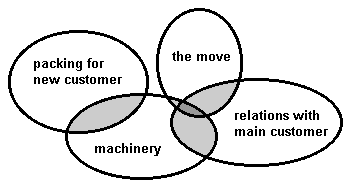
\includegraphics[max width=\textwidth]{3stp7we}
\end{center}

This illustrated the main activities and how they overlapped, and thus gave a good representation of the issues with which System 4 had to deal.

\section*{DRAWING THE VSM - From Step 6 - adding System 4}

\subsection*{Step 6: IDENTIFICATION OF SYSTEM 4 - examples}
You have now drawn in System 4 on your VSM diagram.

Examples of System 4 are as follows:

\subsection*{System 4 - Suma 1991}
Future planning is given occasional consideration by groups and individuals. The Futures committee looked at possibilities for diversystem-in-focusication but didn't produce any proposals. A recent five year plan decided only to continue to proceed in same mode. In summary, there is no continuous focus for System 4 activity, and thus very little future planning.

\subsection*{System 4 - Mondragon}
Mondragon has a firm commitment to Research and Development; its System 4 keeps in touch with developments in all aspects of robotics, production techniques, new products, and computerisation.

Mondragon has built its own R \& D facility.

It is in touch with those aspects of its external environment which may exhibit novelty (e.g. European Space Project).

It is currently looking seriously towards the unified European market in 1993 and planning accordingly.

\section*{Step 7: SYSTEM 5}
PURPOSE: To identify those parts of the System-in-Focus which are concerned with Policy.

Policy concerns the ground rules which affect everyone in an organisation.

In the Viable System, policy is the domain of System 5. It may best be described as "Top Level Ethos", and its role is to become involved in the complex interactions between Systems 3 and 4.

System 5 has two main functions:

Firstly, to supply "logical closure": The loop between systems 3 and 4 is potentially unstable and must be overseen Metasystemically.

Secondly, to monitor the goings on in the whole organisation. These must be constrained by policy.

There is, of course, nothing to stop System 5 wielding its own authority (for example ... demanding that System 4 begins to study a particular issue and that System 3 responds to this ... and that the eventual outcome is passed to the Operational units to be elaborated into a production plan) but this is a rare occurrence.

System 5 provides the context, the ground rules, the ethos.

Who is System 5???

If your mind works like most of us the answer to this question will be something like Henry Ford or Walt Disney or some other hero who dominates the policy of the enterprise. (Any colour as long as it's black ...). Beer has written at length about the way that all elements of the Viable System are mutually dependant, and that giving one any more importance than another is clearly wrong. (How viable would Aristotle have been if any of his major organs had closed down??) The question of who System 5 actually is has to be answered very simply as everyone involved in the system. At the governmental level it should be described as "the Will of the People", within the co-operative it's the same and systems must be designed to ensure that's how it works. (Again notice that Mondragon seem to have grasped the essence .. they describe their General Assembly as "The Will of the Members").

At Suma, the Hub/Sector system evolved to provide a means of ensuring that policy can involve all members on a continuous basis. To my knowledge this is the only System 5 which works in this way with large numbers: usually systems will involve a few meeting a year.

\section*{DRAWING THE VSM - from Step 7 - adding System 5}

\section*{Step 7: SYSTEM 5 - examples}
\textbf{You have now drawn in System 5 on your VSM diagram}

\textbf{Examples of System 5 are as follows:}


\section*{REVIEW: THE VSM IN ITS ENTIRETY}

\section*{Step 8: PRELIMINARY DIAGNOSIS}
By now you have:

\begin{itemize}
  \item Listed the Operational elements.

  \item Identified System 2.

  \item Listed the five functions of System 3 and identified it.

  \item Listed System 4 activities and considered who does them.

  \item Considered policy and the extent to which it represents the views of the members.

\end{itemize}

You have also put all of this together on a large VSM diagram, which will give a picture of your System-in-Focus in its totality.

Now cross out those parts of your organisation which appear on the VSM from your original list.

Remember to be clear about the System-in-Focus. Anything about the internal workings of the Operational elements should not appear on this diagram. (So .. in Suma's case .. the optimisation techniques used within each department don't appear. They are the concern of the next (smaller) level of organisation. The boxes 2, 3, 4 and 5 refer to the whole of Suma.)

If you can't put anything in some of the boxes, you are in the same position that I was. There was effectively no System 4, except when it was unavoidable, at Suma.

At this point you should take some time to consider the implications of the preliminary diagnosis.

Some of the five functions will be performed by people or departments which clearly don't have the resources to do the job adequately.

In some cases the entire Metasystem will be performed informally, and that may be fine (See Case Study on HWMC).

There will be some jobs which are left on your list after filling in the VSM. Are they necessary? Some will be support jobs, like machine maintenance. The computer department is a facilitator, which makes things happen more smoothly and quickly. Both these jobs are clearly useful.

But what about some of the committees? Are they really essential to viability?

**At the end of this process you should have

\begin{itemize}
  \item Identified the major parts of your System-in-Focus which render it viable.

  \item Considered the parts which seem to be inadequate.

  \item Identified any parts which don't map onto the VSM and therefore don't have anything to do with viability.

\end{itemize}

This concludes the Preliminary Diagnosis.

**